% Chapter mq, part E: the family in Thorin form. Source: misc/reviews/nick-allv2/nested_family_M_thorin_for_vadim/family_M_thorin_for_vadim/chapter_family_M_thorin.tex. Reports: misc/research/directions/opus/vol3/FAM.md (14 MAJOR, merge plan), misc/research/directions/astra/FAM/report.md (10 MAJOR, disposition of the six problems), recomputation misc/vol3/verify/FAM/fam.md (our values are used where they differ from the source). Dropped: the theorem with the pairwise proviso, the window proposition resting on the draft [Rub26], the sample table to 4e9 and the claims beyond 1e8.
\section{The inequality (M), Part E: the family in Thorin form}\label{mqf:sec:parte}

This part treats the family of four characters of Part A for a fixed pair $(q,d)$, in the language of the Thorin programme of Part D. The pair is fixed here, whereas in (M) of Part A the pair moves with the window; the statement for one pair is called the \emph{one sided bound for the pair}, and it is not (M) (Proposition~\ref{mq:prop:onesided}). The working draft \cite{Rub26} is unrefereed, and what we attribute to it is reported, not verified. Everything computed below is floating point arithmetic on the stated range, and not a theorem.

\subsection{The family and the sign}\label{mqf:sub:family}

Let $q\equiv3\pmod8$ and $d\equiv7\pmod{16}$ be primes with $q\mid d+1$ (Section~\ref{mq:sec:setting}, Lemma~\ref{mq:lem:congruence}), $\chi_q$ and $\chi_d$ the Legendre symbols, and $\kappa=\pm1$ a sign. The sign is written $\kappa$ because $\epsilon$ is the small parameter of (M). The weight is $w_\kappa=(1+\kappa\chi_q)(1-\chi_d)\ge0$. Write $P_\kappa$ for the two characters with coefficient $+1$ and $N_\kappa$ for the two with coefficient $-1$:
\[
P_+=\{1,\chi_q\},\ N_+=\{\chi_d,\chi_q\chi_d\};\qquad P_-=\{1,\chi_q\chi_d\},\ N_-=\{\chi_d,\chi_q\}.
\]
The sign of \cite{Rub26} is reported to be $\kappa=+1$ (the weight of (M)); $\kappa=-1$ serves as a comparison (Remark~\ref{mql:rem:secondweight}). Since $q\mid d+1$ we have $\chi_d(q)=1$ by reciprocity and $\chi_d(2)=1$, so $w_\kappa$ vanishes on the powers of $2$ and of $q$. The pair $(3,23)$ is the smallest admissible pair, and for $q=3$ the admissible primes are $d\equiv23\pmod{48}$.


For a primitive real $\chi$ of conductor $k$ and parity $a\in\{0,1\}$ let $\xi_\chi(s)=(k/\pi)^{s/2}\Gamma(\frac{s+a}2)L(s,\chi)$ (the usual $\xi$ for the trivial character) and $m_\chi(\lambda)=\frac{\xi_\chi'}{\xi_\chi}(\frac12+\lambda)$. As in equation~\eqref{mq:eq:cchi}, $c_\chi=2m_\chi(\frac12)=\log\frac k\pi+\psi(\frac{1+a}2)+2\frac{L'}L(1,\chi)$ for $\chi\ne1$, and $c_1=2+\gamma_E-\log4\pi$. If the zeros are $\frac12\pm i\gamma$, with $L(\frac12,\chi)\ne0$, then $c_\chi=\sum_{\gamma>0}2/(\frac14+\gamma^2)$. Put $C_{q,d}=\sum_\chi c_\chi$ over the four characters and $C_N=\sum_{\chi\in N_\kappa}c_\chi$.

\subsection{Explicit formulas and the exact slack}\label{mqf:sub:explicit}

Let $S_\chi(x)=\sum_n\chi(n)\Lambda(n)(x/n-1)_+$, and let $\mathrm{tr}(x)=\sum_{k\ge1}x^{-2k}/(2k(2k+1))$ and $\mathrm{tr}_1(x)=\sum_{k\ge1}x^{-(2k-1)}/((2k-1)2k)$ be the trivial zero terms.

\begin{lemma}[Explicit formulas]\label{mqf:lem:explicit}
For $x\ge1$,
\[
\begin{aligned}
S_1(x)&=x\log x-(1+\gamma_E)x+\log2\pi+\Sigma_1(x)-\mathrm{tr}(x),\\
S_\chi(x)&=-x\tfrac{L'}{L}(1,\chi)+\tfrac{L'}{L}(0,\chi)+\Sigma_\chi(x)-\mathrm{tr}_1(x)&&(\chi\ \text{odd}),\\
S_\chi(x)&=-x\tfrac{L'}{L}(1,\chi)+\log x+1+B_\chi+\Sigma_\chi(x)-\mathrm{tr}(x)&&(\chi\ \text{even}),
\end{aligned}
\]
where $\Sigma_\chi(x)=\sum_\rho x^\rho/(\rho(1-\rho))$ over the nontrivial zeros with multiplicity and $B_\chi=L''(0,\chi)/(2L'(0,\chi))$.
\end{lemma}

\begin{proof}
The Mellin transform of $S_\chi$ is $-\frac{L'}L(s,\chi)/(s(s-1))$. The terms are the residues at $s=1$, at $s=0$ (a double pole for an even character), at the nontrivial zeros and at the trivial zeros. This is the exact form of the explicit formula of equation~\eqref{mq:eq:Gpsi}, with no $O(\log x)$.
\end{proof}

Define $H_\chi(u)$ by $\sqrt x\,H_\chi(u)=\Sigma_\chi(x)$, $x=e^u$. Let $\mathrm{main}_\kappa$ be the terms of the lemma other than the sums over zeros, combined with the signs of $w_\kappa$, and $S_{w_\kappa}=\sum_\chi\varepsilon_\chi S_\chi$, with $\varepsilon_\chi=\pm1$ the coefficient of $\chi$ in $w_\kappa$. Put
\[
\Phi_\kappa(u)=\sum_{\chi\in P_\kappa}\bigl(c_\chi-H_\chi(u)\bigr)+\sum_{\chi\in N_\kappa}\bigl(c_\chi+H_\chi(u)\bigr).
\]
Then, unconditionally, $S_{w_\kappa}(x)=\mathrm{main}_\kappa(x)+\sqrt x\,(C_{q,d}-\Phi_\kappa(\log x))$. This sharpens Proposition~\ref{mql:prop:twosided}, whose $O(\log x)$ is replaced by the exact terms. The one sided bound for the pair, for the GRH constant, is $\Phi_\kappa\ge0$.

\begin{proposition}[Slack of the family]\label{mqf:prop:slack}
Assume GRH for the four functions and $L(\frac12,\chi)\ne0$ for the four characters. Then
\[
\Phi_\kappa(u)=\sum_{\chi\in P_\kappa}\sum_{\gamma>0}\frac{4\sin^2(\frac12\gamma u)}{\frac14+\gamma^2}+\sum_{\chi\in N_\kappa}\sum_{\gamma>0}\frac{4\cos^2(\frac12\gamma u)}{\frac14+\gamma^2},
\]
so $0\le\Phi_\kappa\le2C_{q,d}$, and $S_{w_\kappa}(x)\le\mathrm{main}_\kappa(x)+C_{q,d}\sqrt x$. The constant $C_{q,d}$ is the GRH constant. It is best possible if and only if $\inf\Phi_\kappa=0$, which is the condition of Proposition~\ref{mqf:prop:kronecker} below; this holds if the ordinates are linearly independent, and we do not claim it.
\end{proposition}

If a function has a central zero of order $r$, the formula changes by $8r$ for a function of $N_\kappa$ and the mean of $\Phi_\kappa$ becomes $C_{q,d}-4(r_P-r_N)$; for $(3,23)$ no central zero occurs (see below), and we carry the hypothesis in each statement where it is used. The result agrees with Remark~\ref{mql:rem:landau}: GRH for the four functions implies the one sided bound, and the converse is not known (Theorem~\ref{mqf:thm:nocaveat}).

\subsection{The pair $(3,23)$}\label{mqf:sub:pair}

For $q=3$, $d=23$ the conductors are $3$, $23$, $69$. The constants from the functional equation and, independently, from Lemma~\ref{mqf:lem:explicit} at $x=1$ agree (computed):
\begin{center}
\begin{tabular}{lrrr}
\hline
character & conductor & $\frac{L'}{L}(1,\chi)$ & $c_\chi$\\
\hline
trivial & $1$ & & $0.04619$\\
$\chi_3$ & $3$ & $0.36828$ & $0.11323$\\
$\chi_{23}$ & $23$ & $-0.42212$ & $0.56931$\\
$\chi_3\chi_{23}$ & $69$ & $0.05652$ & $1.23891$\\
\hline
\end{tabular}
\end{center}
Here $\frac{L'}{L}(0,\chi)=0.94820$ for $\chi_3$, $-0.29828$ for $\chi_{23}$, and $1+B_\chi=-0.87554$ for $\chi_3\chi_{23}$. The sum is $C_{3,23}=1.96764$ (to five decimals, from $1.9676400683\ldots$), and $2C_N=3.61644$ for $\kappa=+1$. Since every $c_\chi$ is below $4$ and a real zero $\beta\in(0,1)$ would add $1/(\beta(1-\beta))\ge4$ to $c_\chi$ (every other zero adds a positive amount), none of the four functions has a real zero in $(0,1)$ and none has a central zero. This is a one line alternative to Proposition~\ref{mqf:prop:kernels} below and works only for small conductors.

The linear and constant terms of $\mathrm{main}_\kappa$ are (to seven decimals, from the exact expressions)
\[
\begin{aligned}
\mathrm{main}_+(x)&=x\log x-A_+x-\log x+K_+,\\
\mathrm{main}_-(x)&=x\log x-A_-x+\log x+K_-+2(\mathrm{tr}_1-\mathrm{tr})(x),\\
{}&A_+=2.3110956,\ K_+=3.9598929,\ A_-=1.6875777,\ K_-=0.3124223,
\end{aligned}
\]
the trivial zero terms cancelling for $\kappa=+1$ and giving $2(\mathrm{tr}_1-\mathrm{tr})(x)=2(1+x)\log(1+1/x)-2\le2\log2/x$ for $\kappa=-1$.

\begin{corollary}[Explicit form for $(3,23)$]\label{mqf:cor:explicit}
Assume GRH for $\zeta$, $L(s,\chi_3)$, $L(s,\chi_{23})$ and $L(s,\chi_3\chi_{23})$. Then for all $x\ge1$,
\[
\begin{aligned}
S_{w_+}(x)&\le x\log x-2.31109\,x+1.96765\sqrt x-\log x+3.95990,\\
S_{w_-}(x)&\le x\log x-1.68757\,x+1.96765\sqrt x+\log x+0.31243+\frac{2\log2}x,
\end{aligned}
\]
with $S_{w_\pm}(x)=\sum_n(1\pm\chi_3(n))(1-\chi_{23}(n))\Lambda(n)(x/n-1)_+$. The linear coefficients are rounded down and the constants up, so each bound is weaker than the exact one. Conversely, with the exact coefficients of $x$ and of the constant term, either inequality with $C_{3,23}\sqrt x$ replaced by $O_\delta(x^{1/2+\delta})$ for every $\delta>0$ holds if and only if $\nu_\kappa(\rho)=0$ for every zero $\rho$ off the line (Theorem~\ref{mqf:thm:nocaveat}), which is implied by GRH for the four functions and is not known to imply it.
\end{corollary}

\begin{proof}
The coefficient of $x$ is $-(1+\gamma_E+\kappa\frac{L'}L(1,\chi_3)-\frac{L'}L(1,\chi_{23})-\kappa\frac{L'}L(1,\chi_3\chi_{23}))$, the constant is $\log2\pi+\kappa\frac{L'}L(0,\chi_3)-\frac{L'}L(0,\chi_{23})-\kappa(1+B)$, and the coefficient of $\log x$ is $-\kappa$. The sums over zeros are at most $C_{3,23}\sqrt x$ in modulus. The rounding is in the safe direction: the exact bound has $-A_\kappa x$ and $+K_\kappa$, and $A_+>2.31109$, $K_+<3.95990$, $A_->1.68757$, $K_-<0.31243$, $C_{3,23}<1.96765$. A rounding of $A_\kappa$ upward is not allowed: an error proportional to $x$ cannot be repaired by the $\sqrt x$ term.
\end{proof}

\subsection{The slack computed from the primes}\label{mqf:sec:slack}

From the primes (all prime powers of positive weight, $L'/L$ at $s=1$ from the Hurwitz zeta function to $60$ digits, sums in extended precision with unit roundoff $2^{-64}$) we computed $\Phi_+$ and $\Phi_-$ for $(3,23)$ at the prime powers and at the extrema between them, on $1\le x\le2\cdot10^6$ and then on $1\le x\le4\cdot10^9$. This is a floating point computation and not a theorem. On $1\le x\le2\cdot10^6$ we find the following.
\begin{itemize}
\item $\Phi_+\ge0.62559$, with the least value at $x=1354582$, and $\Phi_+\le3.61644=2C_N$, attained at $x=1$. On $0.3\le u\le14.5$ ($e^{0.3}\le x\le2\cdot10^6$) the largest value of $\Phi_+$ is $2.997$ and that of $\Phi_-$ is $2.877$.
\item $\Phi_-\ge0.96266$, with the least value at $x=2512.7$.
\end{itemize}
On the whole range $1\le x\le4\cdot10^9$ the same minima hold (the minimum of $\Phi_+$ is $0.62559$ at $x=1354582$, that of $\Phi_-$ is $0.96266$ at $x=2512.7$), both slacks are positive, and the largest value of $\Phi_-$ is $3.135$, at $x=3.41\cdot10^9$. We have no computation beyond $4\cdot10^9$ and make no claim there.
The normalised error $(S_{w_\kappa}-\mathrm{main}_\kappa)/\sqrt x=C_{3,23}-\Phi_\kappa$ lies in $[-1.030,\,1.342]$ for $\kappa=+1$ and $[-0.909,\,1.005]$ for $\kappa=-1$ on $0.3\le u\le14.5$.

\begin{figure}[ht]
\centering
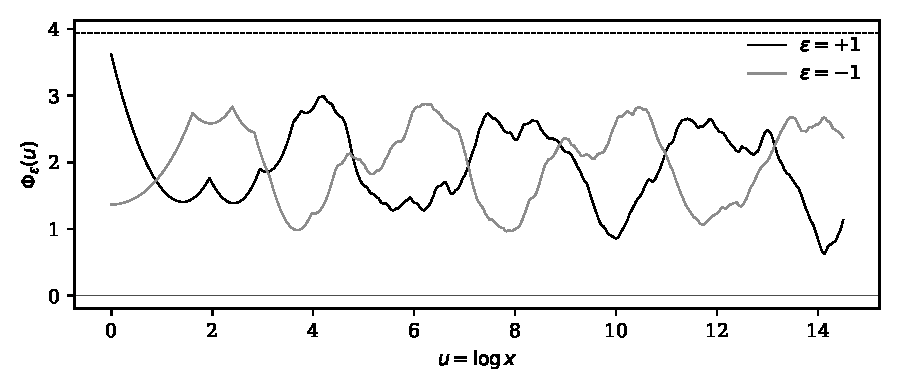
\includegraphics[width=\textwidth]{fig/fam_slack.pdf}
\caption{The slack $\Phi_\kappa$ of the family for $(q,d)=(3,23)$, from the primes up to $2\cdot10^6$, for the two signs. The dashed line is $2C_{3,23}$; the one sided bound for the pair is the statement that the curve stays above $0$.}\label{mqf:fig:slack}
\end{figure}

\paragraph{Mean and spread.} Under GRH and central nonvanishing the mean of $\Phi_\kappa$ over long ranges of $u$ is $C_{q,d}$, and its variance is $\frac12\sum a_\gamma^2$ over distinct ordinates $\gamma$, where $a_\gamma$ is the net weight $2(\sum_Pm_\chi(\gamma)-\sum_Nm_\chi(\gamma))/(\frac14+\gamma^2)$ (a shared ordinate can cancel). Sampled uniformly in $u$ for $10^4\le x\le4\cdot10^9$, the mean and standard deviation are $1.92$ and $0.59$ for $\kappa=+1$ and $2.00$ and $0.58$ for $\kappa=-1$, so $C_{3,23}$ is about $3.4$ standard deviations above $0$. The distribution of the values like a sum of independent terms with uniform phases needs the linear independence of the ordinates and is a model.

\subsection{Slope at the origin and the first arc}\label{mqf:sub:firstarc}

The weight $w_+$ vanishes at $2,3,4,5$ and its first prime power is $7$; $w_-$ vanishes at $2,3,4$ and its first prime is $5$. Below these points the statistic is zero and the slack is elementary.

\begin{proposition}[The first arc for $\kappa=+1$]\label{mqf:prop:firstarc}
For $(3,23)$ and $0\le u<\log7$,
\[
\Phi_+(u)=C_{3,23}+(u-A_+)\,e^{u/2}+(K_+-u)\,e^{-u/2},
\]
positive on this interval, with $\Phi_+(0)=C_{3,23}-A_++K_+=2C_N=3.61644$, right derivative $\Phi_+'(0^+)=-\frac12(A_++K_+)=-3.1355$ and minimum $1.404$ at $u=1.415$. So the first inequality of Corollary~\ref{mqf:cor:explicit} holds, with the exact constants, for $1\le x<7$.
\end{proposition}

\begin{proof}
For $x<7$ the sum over primes is empty, so $\sqrt x(C_{3,23}-\Phi_+)=-\mathrm{main}_+(x)$. For the minimum, $2e^{u/2}\Phi_+'(u)=e^u(u+2-A_+)+u-K_+-2$ is increasing, since its derivative is $e^u(u+3-A_+)+1>0$, and its zero lies in $(1.41,1.42)$.
\end{proof}

The singular behaviour differs from that of $\zeta$ alone. For one function the slack behaves like $\frac12u\log(1/u)$ at the origin (Proposition~\ref{mql:prop:helixprime}). In the family the two functions with coefficient $+1$ contribute $+2\cdot\frac12u\log(1/u)$ and the two with coefficient $-1$ contribute $-2\cdot\frac12u\log(1/u)$, since $c+H=2c-(c-H)$, and the singular parts cancel, so $\Phi_\kappa$ has a finite right derivative at $0$. The cancellation needs as many functions of each sign, counted with the degree of the Gamma factor; it holds for $(1\pm\chi_q)(1-\chi_d)$ and fails for a weight such as $1+\chi_d$.

\begin{proposition}[The slope at the origin]\label{mqf:prop:slope}
Let $q\ne d$ be primes with $q\equiv d\equiv3\pmod4$, and let $A_\kappa$ and $K_\kappa$ be the coefficient of $-x$ and the constant term of $\mathrm{main}_\kappa$. Then $A_++K_+=2\log d$ and $A_-+K_-=2$, and the right derivative at $0$ is $-\frac12\log(k_N/k_P)$, where $k_P,k_N$ are the products of the conductors of the two groups: $\Phi_+'(0^+)=-\log d$ and $\Phi_-'(0^+)=0$.
\end{proposition}

\begin{proof}
The functional equation gives $\frac{L'}L(1,\chi)+\frac{L'}L(0,\chi)=\log2-\log(k/\pi)+\gamma_E$ for odd $\chi$, and the same with $B_\chi$ in place of $\frac{L'}L(0,\chi)$ for even $\chi$. Insert these in $A_\kappa$ and $K_\kappa$: the terms $\log2$ and $\gamma_E$ cancel against $\log2\pi$, $1+\gamma_E$ and the constants of the even character, and the conductors are left as $\log(d\cdot qd/q)$ for $\kappa=+1$ and $\log(q\cdot d/qd)$ for $\kappa=-1$. For $\kappa=-1$ the sum is $2$: it is the $1$ of $1+\gamma_E$ plus the $1$ of $1+B_\chi$. For the slope, the elementary part $(u-A)e^{u/2}+(K+u)e^{-u/2}$ has slope $2-(A_-+K_-)/2=1$ at $0$ when $\kappa=-1$, and the trivial zero term $2(\mathrm{tr}_1-\mathrm{tr})(e^u)e^{-u/2}$ has slope $2\log2-2-(2\log2-1)=-1$. The total is $0$. For $\kappa=+1$ the trivial zeros cancel.
\end{proof}

\subsection{Positivity of the theta kernels for $(3,23)$}\label{mqf:sub:kernels}

Part B (Section~\ref{mql:sub:choice}) defines the theta kernel $\theta_D$ and certifies the positivity for $(3,23)$ in Remark~\ref{mql:comp:pairs}. The following elementary proof, by hand, is placed here so that its application to $(3,23)$ in Theorem~\ref{mqf:thm:nocaveat} does not depend on the interval computation.

\begin{proposition}[Positivity of the three kernels]\label{mqf:prop:kernels}
The theta kernels $\theta_\chi(x)=\sum_{n\ge1}n^a\chi(n)e^{-\pi n^2x/k}$ of $\chi_3$, $\chi_{23}$ and $\chi_3\chi_{23}$ are positive for all $x>0$.
\end{proposition}

\begin{proof}
For a real primitive character $\theta_\chi(1/x)=x^{a+1/2}\theta_\chi(x)$, so take $x\ge1$. Put $y=e^{-\pi x/k}\in(0,y_0]$, $y_0=e^{-\pi/k}$, and $\theta_\chi=y\,g(y)$, $g(y)=\sum_{n\ge1}n^a\chi(n)y^{n^2-1}$. We show $g>0$.

\emph{Conductor $3$.} Here $y_0=0.351$ and $g(y)=1-2y^3+4y^{15}-\cdots\ge1-2y_0^3-\sum_{n\ge5}ny_0^{n^2-1}>1-0.087-10^{-9}$.

\emph{Conductor $23$.} Here $y_0=0.8724$, and the values of $\chi_{23}$ at $1,\dots,9$ are $+,+,+,+,\allowbreak-,+,-,\allowbreak+,+$, so
\[
g(y)\ \ge\ 1+\bigl(4y^{15}-5y^{24}\bigr)+\bigl(6y^{35}-7y^{48}\bigr)-\sum_{n\ge10}ny^{n^2-1},
\]
the terms with $n=2,3,8,9$ being positive and dropped. Now $4y^{15}-5y^{24}=y^{15}(4-5y^9)\ge0$ since $y_0^9=0.293$, and $6y^{35}-7y^{48}=y^{35}(6-7y^{13})\ge0$ since $y_0^{13}=0.170$. For the tail, $n^2-100\ge21(n-10)$ for $n\ge10$, so with $r=y_0^{21}=0.057$ it is at most $y^{99}(10/(1-r)+r/(1-r)^2)\le10.7\,y_0^{99}<2\cdot10^{-5}$. Hence $g>0.9999$.

\emph{Conductor $69$.} Here $a=0$, $y_0=0.9555$, and the values of $\chi_{69}$ at $1,\dots,9$ are $+,-,0,+,+,0,-,-,0$, so
\[
g(y)\ \ge\ \bigl(1-y^3\bigr)+\bigl(y^{15}-y^{48}\bigr)+\bigl(y^{24}-y^{63}\bigr)-\sum_{n\ge10}y^{n^2-1}.
\]
The first and third brackets are positive. For the second, $y^{15}-y^{48}=y^{15}(1-y^{33})\ge0.777\,y^{15}$ since $y_0^{33}=0.223$. The tail is at most $y^{99}/(1-y_0^{21})\le1.63\,y^{99}$, and $1.63\,y^{99}\le0.777\,y^{15}$ because $y^{84}\le y_0^{84}=0.022$. Hence $g>0$.
\end{proof}

On a grid the minimum of $g$ on $(0,y_0]$ is $0.914$, $1.000$ and $0.493$ in the three cases (computed). The same grid computation for the other admissible pairs with small conductors gives the table below. For every pair the minimum for $\chi_d$ is $1.000$ (since $g\to1$ at $0$ and $\chi_d$ has no early negative term), and the table gives the minimum for the product character $\chi_q\chi_d$, the constants and the first prime that carries weight.
\begin{center}
\small
\begin{tabular}{lrrrr}
\hline
pair & $\min g_{\chi_q\chi_d}$ & $C_{q,d}$ & $2C_N$ ($\kappa=+1$) & first prime\\
\hline
$(3,23)$ & $0.493$ & $1.9676$ & $3.616$ & $7$\\
$(3,71)$ & $-0.330$ & $3.8005$ & $7.282$ & $7$\\
$(3,263)$ & $-0.008$ & $5.492$ & $10.666$ & $7$\\
$(11,263)$ & $0.684$ & $6.436$ & $11.764$ & $5$\\
$(19,151)$ & $0.689$ & $6.347$ & $10.496$ & $7$\\
\hline
\end{tabular}
\end{center}
The entries are minima on a grid of $4\cdot10^5$ points and are not proved, except for $(3,23)$. For $(3,71)$ and $(3,263)$ the product kernel is negative on the grid, which does not mean that the product character has a real zero. The computed zeros of Platt \cite{Platt16} (low zeros on the line for the conductors of the table, and central nonvanishing), as we read them, exclude real zeros in $(0,1)$ for these conductors even when a kernel changes sign; we have not rechecked that reading, and it gives no positivity of a sign changing kernel and no information on zeros of large height. Pairs with sign changing kernels are therefore not excluded from Theorem~\ref{mqf:thm:nocaveat}, whose hypothesis is only the absence of real zeros of the two functions of $N_\kappa$.

\subsection{Net multiplicities}\label{mqf:sub:nocaveat}

For a complex $\rho$ let $\nu_\kappa(\rho)$ be the sum of the multiplicities of $\rho$ as a zero of the functions of $P_\kappa$ less the sum for the functions of $N_\kappa$. The following is the form of Proposition~\ref{mq:prop:onesided}(1) for the family, with the real point hypothesis replaced by the kernels, and it is the only equivalence we state.

\begin{theorem}[The one sided bound and net multiplicities]\label{mqf:thm:nocaveat}
Suppose neither function of $N_\kappa$ has a zero in $(0,1)$ (this holds if the theta kernels of the two characters of $N_\kappa$ are positive, and then $\xi_\chi>0$ on the real axis). The following are equivalent.
\begin{enumerate}
\item[(a)] For every $\delta>0$, $S_{w_\kappa}(x)\le\mathrm{main}_\kappa(x)+O_\delta(x^{1/2+\delta})$.
\item[(b)] $\nu_\kappa(\rho)=0$ for every nontrivial $\rho$ off the critical line.
\item[(c)] $\Phi_\kappa(u)\ge0$ for all $u>0$.
\end{enumerate}
When they hold, $\Phi_\kappa(u)=\sum_P\sum_\gamma w_\gamma(1-\cos\gamma u)+\sum_N\sum_\gamma w_\gamma(1+\cos\gamma u)+2T_N+8r_N$, the sums being over the zeros on the line (the central zeros, of total order $r_N$ in $N_\kappa$, entering through $8r_N$), and $T_N\ge0$ the sum of $1/(\rho(1-\rho))$ over the zeros of the functions of $N_\kappa$ off the line.
\end{theorem}

\begin{proof}
(c) implies (a) trivially. (a) implies (b) by the signed Landau argument of Proposition~\ref{mq:prop:onesided}: the transform of the nonnegative function $\mathrm{main}_\kappa+Bx^{1/2+\delta}-S_{w_\kappa}$ is analytic to the right of its first real singularity, a real point $\beta$ with $\nu>0$ gives a pole with negative residue $-\nu(\beta)/(\beta(1-\beta))$, which a nonnegative function cannot have at its abscissa, and a real point with $\nu<0$, which could, does not occur because the functions of $N_\kappa$ have no real zero in $(0,1)$. So the transform is analytic in $\Re s>\frac12+\delta$ for every $\delta>0$, and its poles there are the points with $\nu_\kappa(\rho)\ne0$. The functional equation gives the same for $\Re\rho<\frac12$. For (b) implies (c), write $\Phi_\kappa=C_{q,d}-D_\kappa$ with $D_\kappa=\sum_PH_\chi-\sum_NH_\chi$ as a sum over zeros. The contribution of each $\rho$ off the line to $D_\kappa$ is $\nu_\kappa(\rho)x^{\rho-1/2}/(\rho(1-\rho))=0$, and since $c_\chi=\sum_\rho1/(\rho(1-\rho))$ over all zeros, by (b) the zeros off the line contribute the same amount $T_N$ to $\sum_Pc_\chi$ and to $\sum_Nc_\chi$. A central zero contributes $4r$ to $c_\chi$ and $4r$ to $H_\chi$. This gives the formula. Finally $T_N\ge0$, because for $\rho=\beta+i\gamma$ in the strip the sum of $1/(\rho(1-\rho))$ over $\rho$ and $\bar\rho$ is $2(\beta(1-\beta)+\gamma^2)/|\rho(1-\rho)|^2>0$.
\end{proof}

So the one sided bound for the pair is equivalent to the statement that the quotient $\prod_PL/\prod_NL$ has no zero and no pole off the line, counted with net multiplicity (condition (b)). GRH for the four functions implies it, and the converse needs the exclusion of a zero off the line shared by the two groups with equal total multiplicity (for instance multiplicities $(1,1,2,0)$ for $\zeta,L(\chi_q),L(\chi_d),L(\chi_q\chi_d)$ at a point off the line, which no pair of functions detects). We know of no theorem that excludes such a zero for a fixed pair, and we do not claim that the bound implies GRH, or that the Wald partners have the form $\tau_\chi$. The bound is not Wald partners either: partners imply it, and the converse is not known.

\subsection{Two clocks and the kernel of the family}\label{mqf:sub:clocks}

Under GRH for $\chi$ and $L(\frac12,\chi)\ne0$ the hitting time of Proposition~\ref{mqt:prop:hitting} is $\tau_\chi=\sum_\gamma e_\gamma/(\gamma^2/2)$, with $c_\chi$ the mean of $\tau_\chi$ tilted at rate $\frac18$ (Theorem~\ref{mqt:thm:esscher}). Put $\tau_P=\sum_P\tau_\chi$ and $\tau_N=\sum_N\tau_\chi$, sums of independent times. Then $C_{q,d}=\mathbb E\tau_P^{(1/8)}+\mathbb E\tau_N^{(1/8)}$ and
\[
\Phi_\kappa(u)=\mathbb E\tau_P^{(1/8)}\;\mathbb E\bigl[2\sin^2(\tfrac12\Gamma_Pu)\bigr]+\mathbb E\tau_N^{(1/8)}\;\mathbb E\bigl[2\cos^2(\tfrac12\Gamma_Nu)\bigr],
\]
with $\Gamma_P,\Gamma_N$ drawn with the tilted weights. For $(3,23)$ and $\kappa=+1$ the two means are $0.159$ and $1.808$ (ratio $11.3$, so the clock of the denominator is the slower one and the $\cos^2$ part dominates); for $\kappa=-1$ they are $1.285$ and $0.683$, and only the plus sign has the longer clock in the denominator.

In the language of Wald couples (Theorem~\ref{mqt:thm:wald}), each character with positive theta kernel has a first member $X_\chi$ with $\mathbb E\,e^{\lambda X_\chi}=\xi_\chi(\frac12+\lambda)/\xi_\chi(\frac12)$, unconditionally (for $\zeta$ by Pólya's kernel, Part D). For $\zeta$ the partner exists unconditionally (Theorem~\ref{mqt:thm:wald}); that the partner has the form $\tau_\chi$ is GRH for $\chi$ with the central condition. Under these, the family quotient divided by its value at the centre equals $\mathcal L_{\tau_N}(s)/\mathcal L_{\tau_P}(s)$, the ratio of the Laplace transforms. A difference of Thorin measures need not be a Thorin measure, and a ratio of Laplace transforms does not by itself define an extended generalised gamma convolution \cite{Bondesson}, so no such statement is made. The prime side is nonnegative: $w_\kappa\Lambda\ge0$.

For one function the helix kernel is $c-H(u)-H(v)+H(|u-v|)$. For the family the vectors of the two groups are $e^{i\gamma u}-1$ and $e^{i\gamma u}+1$, and the kernel is
\[
\begin{aligned}K_\kappa(u,v)={}&\sum_{\chi\in P_\kappa}\bigl(c_\chi-H_\chi(u)-H_\chi(v)+H_\chi(|u-v|)\bigr)\\&+\sum_{\chi\in N_\kappa}\bigl(c_\chi+H_\chi(u)+H_\chi(v)+H_\chi(|u-v|)\bigr).\end{aligned}
\]

\begin{proposition}[Structure of the family kernel]\label{mqf:prop:kernel}
Let $\Delta_\kappa=\sum_PH_\chi-\sum_NH_\chi$ and $\mathcal E=\sum_\chi H_\chi$ over all four characters. Then $K_\kappa(u,v)=C_{q,d}-\Delta_\kappa(u)-\Delta_\kappa(v)+\mathcal E(|u-v|)$ and $K_\kappa(u,u)=2C_{q,d}-2\Delta_\kappa(u)=2\Phi_\kappa(u)$. On the side of the primes, $\Delta_\kappa$ is the normalised statistic of the weight $w_\kappa$ of the pair, and $\mathcal E$ is that of the weight $w'=(1+\chi_q)(1+\chi_d)$, the same for both signs. Under GRH for the four functions $K_\kappa$ is positive semidefinite, and the positivity of $K_\kappa$ on $(0,\infty)$ implies $\Phi_\kappa\ge0$.
\end{proposition}

\begin{proof}
Collect terms; on the diagonal $\mathcal E(0)=C_{q,d}$. Under GRH the kernel is a sum of Gram kernels in $L^2$ of the zeros, with positive multiplicity weights and the real part of the inner product. The diagonal is $2(C_{q,d}-\Delta_\kappa)=2\Phi_\kappa$. The weight of $\mathcal E$ is $1+\chi_q+\chi_d+\chi_q\chi_d=(1+\chi_q)(1+\chi_d)$ for either sign, because $\mathcal E$ adds all four $H_\chi$ with coefficient $+1$.
\end{proof}

So the kernel involves two nonnegative weights. The diagonal sees $w_\kappa$ alone; the off diagonal part sees $w'$, the weight of the logarithmic derivative of the Dedekind zeta function of the biquadratic field (with the usual qualification for ramified primes and higher powers; for instance $w_-(23)=2$ and $w_+(23^2)=2$), which carries the primes that split completely. For $(3,23)$ the first prime power of positive weight is $7$ for $w_+$, $5$ for $w_-$ and $3$ for $w'$ (coefficient $2\log3$). Full positivity of the kernel couples it to the other, and by the same Gram argument global positive semidefiniteness of this kernel on the half line is equivalent to individual GRH for the four functions (the transform of $\mathcal E$ has a nonzero residue at every zero to the right of the line, even a shared one).

For $(3,23)$ the matrices on grids of $200$ points in $(0,10]$ and $300$ points in $(0,12]$ are positive definite for both signs, with least eigenvalue about $0.07$ (computed). The archimedean part alone, with the prime sums removed, stays positive on $(0,L)$ up to the grid thresholds $L^*=2.96$ ($e^{L^*}=19.3$, $\kappa=+1$) and $L^*=3.06$ ($e^{L^*}=21.3$, $\kappa=-1$). For $\zeta$ the same computation gives $L^*=0.743$ (Section~\ref{mqt:sub:helix}). These are grid transitions and not proofs.

\subsection{The Thorin form}\label{mqf:sub:thorin}

Let $m_w=\sum_Pm_\chi-\sum_Nm_\chi$. By the Euler products, for $\lambda>\frac12$,
\begin{equation}\label{mqf:eq:mw}
\begin{gathered}
m_w(\lambda)=A_w(\lambda)-\sum_{n\ge1}\frac{w_\kappa(n)\Lambda(n)}{n^{1/2+\lambda}},\\
A_w(\lambda)=\frac1{\lambda+\frac12}+\frac1{\lambda-\frac12}+\sum_\chi\varepsilon_\chi\Bigl(\tfrac12\log\tfrac{k_\chi}\pi+\tfrac12\psi\bigl(\tfrac{\frac12+\lambda+a_\chi}2\bigr)\Bigr),
\end{gathered}
\end{equation}
with $\varepsilon_\chi=\pm1$ the coefficient of $\chi$ in $w_\kappa$. So $m_w$ is an explicit archimedean function minus the Dirichlet series of a nonnegative weight; at $\lambda=\frac12$ it is evaluated from the completed logarithmic derivatives.

\begin{theorem}[Thorin form of the one sided bound for the pair]\label{mqf:thm:thorin}
For $b>\frac12$ let $F_w(b)=\dfrac{b\,m_w(b)-\frac12m_w(\frac12)}{b\,(b^2-\frac14)}+\dfrac{2C_N}b$. Then $F_w(b)=\int_0^\infty e^{-bu}\Phi_\kappa(u)\,du$ for $b>\frac12$, and $\Phi_\kappa\ge0$ holds if and only if $F_w$ is completely monotone on $(\frac12,\infty)$.
\end{theorem}

\begin{proof}
For one function $\int_0^\infty e^{-bu}(c_\chi-H_\chi(u))du=(b\,m_\chi(b)-\frac12m_\chi(\frac12))/(b(b^2-\frac14))$, as in Theorem~\ref{mqt:thm:esscher}; the integral converges for $b>\frac12$ because every zero has real part below $1$. For a function of $N_\kappa$ the integrand is $c_\chi+H_\chi$, with transform $2c_\chi/b$ minus that of $c_\chi-H_\chi$. Add. The equivalence is Bernstein's theorem applied to $F_w(b_0+t)$, $t>0$, with the continuity of $\Phi_\kappa$.
\end{proof}

Without hypothesis $bF_w(b)\to\Phi_\kappa(0)=2C_N$ as $b\to\infty$ (initial value theorem, $\Phi_\kappa$ being continuous at $0$); under GRH and central nonvanishing $bF_w(b)\to C_{q,d}$ as $b\to0^+$ (mean value of an almost periodic function). For $(3,23)$ and $\kappa=+1$ these are $3.616$ and $1.968$ (computed).

\begin{problem}[(E$_{q,d,\kappa}$), Thorin form]\label{mqf:prob:thorin}
For primes $q\equiv3\pmod8$, $d\equiv7\pmod{16}$ with $q\mid d+1$, and the weight $w_\kappa$, show that the function $F_w$ of Theorem~\ref{mqf:thm:thorin}, which is defined by~\eqref{mqf:eq:mw} from an explicit archimedean function, three constants and the Dirichlet series $\sum w_\kappa(n)\Lambda(n)n^{-s}$ at real $s>1$, satisfies $(-1)^kF_w^{(k)}(b)\ge0$ for all $k\ge0$ and all $b>\frac12$.
\end{problem}

By Theorem~\ref{mqf:thm:nocaveat} this is, under the kernel hypothesis, the statement that the quotient has no zero and no pole off the line counted with net multiplicity. It is stated on the side of the primes: no zero occurs in it. For the window consequence that matters for (M) we do not prove a separate lemma: when the theta kernels of the two characters of $N_\kappa$ are positive no real point has negative net order, and Theorem~\ref{mq:thm:windowcombo} (for the signed combination, with the centring differing from that of Part A by $O(1+\log x)$, harmless on windows) shows that a bound $S_{w_\kappa}(x)-\mathrm{main}_\kappa(x)\le x^\theta$ on windows $[Y,Y^{3/2}]$ for arbitrarily large $Y$ gives $\nu_\kappa(\rho)=0$ for $\theta<\Re\rho<1$. The zeta window is Theorem~\ref{mq:thm:window}.

\paragraph{What a proof in this form would need.} The situation is that of $\zeta$ alone (Section~\ref{mqt:sub:verdict}), with two differences. First, the family has room: $\Phi_\kappa(0)=2C_N$ is $3.6$ for $(3,23)$ and $\kappa=+1$ against a range $[0,2C_{3,23}]=[0,3.94]$, and on the range computed the slack stays above $0.62$. Whether the room persists, $\inf\Phi_\kappa>0$, is a question of simultaneous approximation for the ordinates of four functions (Proposition~\ref{mqf:prop:kronecker}). Second, the arithmetic of the weight enters only through the Dirichlet series in~\eqref{mqf:eq:mw}, with nonnegative coefficients supported on the prime powers of one class of primes. A proof in this form would have to use that support. We have no proof and no mechanism to propose. It is not the inequality that \cite{Rub26} reports: there the pair moves with the window, and the relation to (M) is that of Proposition~\ref{mq:prop:onesided}.

\subsection{The six open problems}\label{mqf:sec:open}

Six problems remain.

\paragraph{1. The convention and the admissible pairs.} As read in \cite{Rub26} (reported, not verified here), the prime sum is $\sum\Lambda(r)(1+\chi_q(r))(1-\chi_d(r))(x/r-1)$, so the sign is $\kappa=+1$ and the further condition $q\mid d+1$ holds. Disposition: this is settled as a matter of reading, and agrees with Lemma~\ref{mq:lem:congruence} and Remark~\ref{mql:rem:secondweight}. The positivity of the kernels is proved here for $(3,23)$ (Proposition~\ref{mqf:prop:kernels}) and is a grid observation for the others. The selection of a pair for each window is Proposition~\ref{mql:prop:choose}.

\paragraph{2. The bound for every $x$.} Write $g_\kappa(x)=\mathrm{main}_\kappa(x)+C_{q,d}\sqrt x-S_{w_\kappa}(x)=\sqrt x\,\Phi_\kappa(\log x)$.

\begin{lemma}[Convexity between the primes]\label{mqf:lem:convex}
Suppose $C_{q,d}<8$ for $\kappa=+1$, or $C_{q,d}<3.2$ for $\kappa=-1$. Between two consecutive prime powers of positive weight $g_\kappa$ is convex. Hence for $a\le x\le b$ with no such prime power strictly between $a$ and $b$
\[
g_\kappa(a)+\min\bigl(0,g_\kappa'(a^+)\bigr)(b-a)\ \le\ g_\kappa(x)\ \le\ \max\bigl(g_\kappa(a),g_\kappa(b)\bigr).
\]
\end{lemma}

\begin{proof}
On such an interval $S_{w_\kappa}$ is linear. For $\kappa=+1$ the second derivative is $x^{-1}+x^{-2}-\frac14C_{q,d}x^{-3/2}$, positive since $x^{1/2}+x^{-1/2}\ge2>\frac14C_{q,d}$. For $\kappa=-1$ it is $x^{-1}-(x-1)/(x^2(x+1))-\frac14C_{q,d}x^{-3/2}$, and $(x-1)/(x(x+1))\le3-2\sqrt2<0.18$, so it is at least $x^{-1}(0.82-\frac14C_{q,d})$.\end{proof}

The sweep of Section~\ref{mqf:sec:slack} used the lemma. It is a floating point computation on $1\le x\le4\cdot10^9$ (the sums are not in interval arithmetic and no independent check was made), so it is not a theorem. Disposition: a certificate (interval arithmetic with directed rounding, with the minimum and the maximum at $x=1$ proved on their intervals, and independent checking) and a larger range are open.

\paragraph{3. Is the infimum of the slack zero?} Under GRH the slack is an almost periodic function, and the question has an exact answer.

\begin{proposition}[Criterion for the infimum]\label{mqf:prop:kronecker}
Assume GRH for the four functions and $L(\frac12,\chi)\ne0$ for $\chi\in N_\kappa$. List the positive ordinates of the zeros of the functions of $P_\kappa$ and of $N_\kappa$, with multiplicity, as $\Gamma_P$ and $\Gamma_N$. Then $\inf_{u>0}\Phi_\kappa(u)=0$ if and only if no ordinate is shared between $\Gamma_P$ and $\Gamma_N$ and every integer relation $\sum n_\gamma\gamma=0$ (finitely many $n_\gamma\ne0$) has $\sum_{\gamma\in\Gamma_N}n_\gamma$ even. Likewise $\sup_u\Phi_\kappa(u)=2C_{q,d}$ if and only if no ordinate is shared and every such relation has $\sum_{\gamma\in\Gamma_P}n_\gamma$ even, under $L(\frac12,\chi)\ne0$ for $\chi\in P_\kappa$.
\end{proposition}

\begin{proof}
By Proposition~\ref{mqf:prop:slack}, $\Phi_\kappa(u)=\sum_{\Gamma_P}w_\gamma(1-\cos\gamma u)+\sum_{\Gamma_N}w_\gamma(1+\cos\gamma u)$ with positive weights of finite sum. For a finite set $F$ of ordinates let $\Phi_F$ be the sum over $F$. Then $\Phi_F\le\Phi_\kappa\le\Phi_F+2\sum_{\gamma\notin F}w_\gamma$, so the infimum of $\Phi_\kappa$ is zero if and only if that of every $\Phi_F$ is. The infimum of $\Phi_F$ is zero if and only if the numbers $\gamma u$ can be brought simultaneously as near as we please, modulo $2\pi$, to $0$ for $\gamma\in\Gamma_P\cap F$ and to $\pi$ for $\gamma\in\Gamma_N\cap F$. By Kronecker's theorem this holds if and only if every integer relation among the $\gamma\in F$ is satisfied by the target, that is $\pi\sum_{\Gamma_N}n_\gamma\equiv0\pmod{2\pi}$. A shared ordinate is the relation $\gamma-\gamma=0$ with odd sum. The supremum is the same with the targets exchanged.
\end{proof}

The criterion is satisfied if the ordinates are linearly independent over $\mathbb Q$, which is expected, and the infimum is then not attained. An almost periodic function returns to within any distance of each of its values on a relatively dense set, so under GRH the computed values give $\liminf_{x\to\infty}\Phi_+(\log x)\le0.6256$ and $\limsup_{x\to\infty}\Phi_+(\log x)\ge2C_N=3.6164$, if the computed minimum is granted. Disposition: the criterion settles the characterisation under GRH; whether the ordinates satisfy it is open.

\paragraph{4. Windows.} Disposition: the fixed pair statement is Theorem~\ref{mq:thm:windowcombo}, quoted in the previous subsection, and the zeta window criterion is Theorem~\ref{mq:thm:window}. The moving pair of \cite{Rub26} has different quantifiers: for each window a pair is chosen, with $\log q$ about $Y^{\epsilon/5}$, and twisted sums are reported there to be bounded directly (proved here as Estimates B and C, Subsection~\ref{mq:sub:BC}), so that the window lemma is applied to $\zeta$ alone. Whether this closes is not a claim of this part.

\paragraph{5. The first prime weight.} For $\zeta$, the positivity of the helix kernel on $(0,L)$ narrows the admissible weight at the prime $2$ to within one per cent of $\log2$ by $L\approx0.93$ (Section~\ref{mqt:sub:helix}, numerical). For the family we replaced the coefficient $4\log7$ of $(x/7-1)_+$ in $S_{w_+}$ by a free number, keeping every other prime at its true value, and asked for which values $K_+$ stays positive semidefinite on a grid of $360$ points in $(0,L)$; the same for the coefficient $2\log3$ of the first prime power of $w'$, entering through $\mathcal E$, and for $\zeta$ at the prime $2$. The admissible intervals, as multiples of the true weight (grid computations, not proofs):
\begin{center}
\small
\begin{tabular}{lcccc}
\hline
$L$ & $e^L$ & weight at $7$ in $w_+$ & weight at $3$ in $w'$ & $\zeta$, weight at $2$\\
\hline

$3.0$ & $20$ & $[0.11,\ 1.17]$ & $[-1.48,\ 1.27]$ & $[0.9993,\ 1.0000]$\\

$7.0$ & $1097$ & $[0.9992,\ 1.0007]$ & $[0.9993,\ 1.0001]$ & $[0.9999,\ 1.0000]$\\
\hline
\end{tabular}
\end{center}
The widths of order $10^{-3}$ are at the resolution of the grid. The family has the same funnel as $\zeta$ but it opens later (Figure~\ref{mqf:fig:funnel}): for $e^L<20$ the kernel on $(0,L)$ is positive even when the prime $7$ is removed or given a negative weight, and the interval reaches a width of one per cent only between $x=150$ and $x=400$ (for $\zeta$ by $x\approx2.5$). Consequently, for the family the step at the first primes is not forced by the arc before it. Disposition: that the interval shrinks to the true weight as $L\to\infty$ is open for the family, with all weights varying; the case of one weight is the rigidity of Part D.

\begin{figure}[ht]
\centering
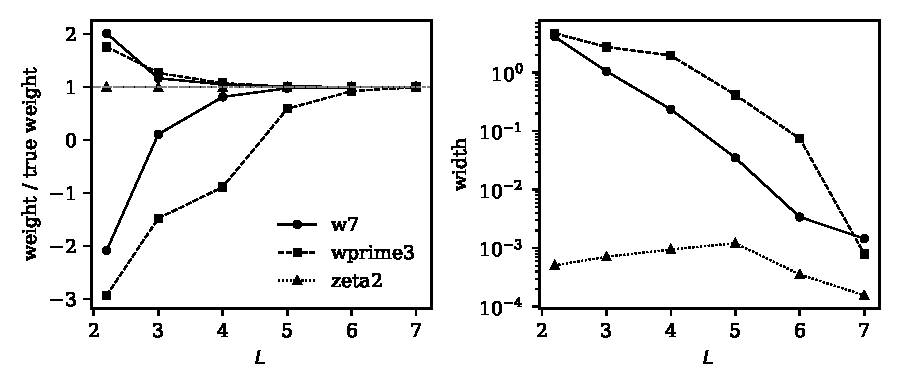
\includegraphics[width=\textwidth]{fig/fam_funnel.pdf}
\caption{The extension problem at the first prime for $(3,23)$. Left: the interval of weights, as a multiple of the true weight, for which the kernel on $(0,L)$ stays positive semidefinite on a grid. Right: the width of the interval.}\label{mqf:fig:funnel}
\end{figure}

\paragraph{6. Common zeros.} Disposition: Theorem~\ref{mqf:thm:nocaveat} is the exact statement for the reduced divisor, with net multiplicities. The exclusion of a shared zero off the line, with equal total multiplicity in the two groups, is open for a fixed pair. Theta positivity settles the real zero issue for $(3,23)$ (Proposition~\ref{mqf:prop:kernels}), and, as we read them (not rechecked here), the computations of \cite{Platt16} settle it for the small pairs of the table.

\paragraph{The regime of Part A, and what remains open.} For $\kappa=+1$ the first arc ends at the least prime $p$ with $\chi_q(p)=1$ and $\chi_d(p)=-1$, which under GRH is $O((\log qd)^2)$. In the regime of Part A, with $\log q$ about $Y^{\epsilon/5}$ and $x\ge Y$, we have $x$ much larger than $(\log qd)^2$, so many prime powers of positive weight lie below $x$ and this is not the first arc; the Dirichlet series in~\eqref{mqf:eq:mw} has infinitely many terms at every real $s>1$. What is true is that $u/\log(qd)\to0$, so that in units of $\log(qd)$ the slack is near its value $2C_N$ at the origin with slope $-\log d$ (Proposition~\ref{mqf:prop:slope}). What remains open: the first $x>1$ at which $\Phi_+$ exceeds $2C_N$ (in every computed case the largest value of $\Phi_+$ is its value at $x=1$, whereas under linear independence the supremum is $2C_{q,d}$), and the description of the slack and of $F_w$ for $u/\log(qd)\to0$ with the conductors tending to infinity.

\subsection{Discussion}\label{mqf:sub:discussion}

At finite range the family is the more comfortable object. This is by design: in \cite{Rub26} the weight is reported to arise because the divisible objects see the inert primes of one field and are sorted by a second character, and the inequality that results is one sided for a nonnegative weight. The price is that the statement concerns four $L$ functions, and its truth for all $x$ requires every zero off the line, if there is one, to be shared by the two groups with equal total multiplicity.

\emph{What the numbers do not say.}
 They say that the one sided bound for $(3,23)$ holds on $1\le x\le4\cdot10^9$ with room, that each of the four functions satisfies its own bound on $x\le2\cdot10^6$, and that the two signs behave alike. They say nothing about RH: a zero off the line at height $T$ with real part $\frac12+\delta$ would add a term of size $x^\delta/T^2$ times its net multiplicity to the normalised statistic, invisible at these ranges unless $T$ is small, and the low zeros of these functions are on the line by the computations cited \cite{Platt16}.
